\documentclass[12pt]{article}
\usepackage[a4paper, margin=1in]{geometry}
\usepackage{times}
\usepackage{graphicx}
\usepackage{tikz}
\usetikzlibrary{shapes.geometric, arrows.meta, positioning, calc}
\usepackage{cite}
\usepackage{setspace}
\usepackage{titlesec}
\usepackage{hyperref}

\onehalfspacing

\titleformat{\section}{\large\bfseries\scshape}{\thesection.}{1em}{}
\titleformat{\subsection}{\normalsize\bfseries}{\thesubsection.}{1em}{}

\begin{document}

\begin{center}
    {\LARGE \textbf{DefectLens: Efficient ViT-Based Anomaly Detection with Multi-Criteria Token Fusion (MCTF)} \par}
    \vspace{0.5cm}
    {\large \textbf{Sachin Singh} \par}
    {\large Roll No: 2023bcs0064 \par}
    {\large Computer Vision Course Project \par}
    {\large Weekly Project Write-Up \par}
    \vspace{0.5cm}
\end{center}

\begin{abstract}
\noindent This report outlines the foundational requirements and architecture for the DefectLens project. It details the core problem of computational inefficiency in Vision Transformers (ViTs) for high-resolution industrial anomaly detection. Furthermore, it explains the motivation behind applying a Multi-Criteria Token Fusion (MCTF) architecture for real-time edge deployment, and the specific objectives the project intends to achieve to solve the stringent accuracy-latency trade-off in modern automated optical inspection systems.
\end{abstract}

\vspace{0.5cm}

\section{Problem Statement}
Industrial visual inspection is paramount for maintaining manufacturing quality control. Traditional supervised learning approaches are fundamentally constrained as they require exhaustively labeled datasets for every conceivable defect type---a practical impossibility given the rarity, subtlety, and unpredictable nature of manufacturing flaws. Consequently, unsupervised anomaly detection---learning the manifold of pristine ``normal'' products---has emerged as the standard paradigm.

While Vision Transformers (ViTs) have achieved state-of-the-art performance in these tasks by capturing comprehensive global context and rich patch-level representations, they inherently suffer from massive computational overhead due to their quadratic complexity with sequence length. In industrial scenarios where high throughput (low latency) and high-resolution imaging are critical, the fixed and highly redundant token processing of standard ViTs introduces a debilitating bottleneck. 

The core problem this project addresses is: \textit{How can we drastically reduce the computational footprint of ViTs for anomaly detection without sacrificing the high-resolution, fine-grained visual details required for accurate defect localization?}

\section{Motivation and Application}
Failing to detect subtle defects can lead to catastrophic product failures, massive recalls, and safety hazards, particularly in precision industries like aerospace, medical devices, and semiconductor manufacturing. Conversely, an overly slow inspection system creates a severe production bottleneck, reducing yield. Resolving the latency-accuracy trade-off is critical for enabling next-generation smart manufacturing and Industry 4.0.

The primary motivation stems from the stringent operational demands of modern manufacturing pipelines, which require inspection mechanisms to be both exceptionally accurate and blisteringly fast. Standard CNN-based models often struggle with complex global geometries and textures, while standard ViTs are too computationally dense for real-time edge deployment on automated production lines.

\textbf{Intended Application:} This project is specifically designed for deployment in Automated Optical Inspection (AOI) systems located directly on factory floors. By leveraging a high-performance, optimized anomaly detection model, manufacturers can instantly identify structural defects, surface contaminations, and assembly errors (comparable to those found in the MVTec AD dataset) in real-time as products move rapidly along a conveyor belt.

\section{Objectives of the Project}
The central objective of DefectLens is to engineer an optimized, high-throughput industrial anomaly detection architecture that harnesses the profound representational power of Vision Transformers while systematically mitigating their computational drawbacks. Specifically, the project intends to achieve the following:

\begin{itemize}
    \item \textbf{Establish a Baseline:} Implement a Vision Transformer architecture coupled with a Memory Bank (PatchCore-style) to create a robust foundation for unsupervised anomaly detection.
    \item \textbf{Develop Dynamic Token Fusion:} Integrate a Multi-Criteria Token Fusion (MCTF) module that dynamically identifies and merges redundant background tokens across ViT layers based on the methodologies proposed by Lee et al. \cite{lee2023multi}.
    \item \textbf{Preserve Critical Data:} Implement specialized criteria---including token similarity, informativeness (via one-step-ahead attention), and token size penalties---to ensure that small but critical defect representations are protected from being erroneously merged.
    \item \textbf{Accelerate Inference:} Drastically reduce the Floating Point Operations (FLOPs) and overall end-to-end latency by reducing token counts, making the model viable for high-speed edge inference.
    \item \textbf{End-to-End System Integration:} Package the model with a functional FastAPI backend and a React-based frontend to simulate a real-world quality control dashboard.
\end{itemize}

\section{System Architecture Diagram}
To achieve the token reduction without accuracy loss, the MCTF module is integrated directly between the Vision Transformer layers. Figure \ref{fig:architecture} demonstrates the high-level workflow of the system from image capture to anomaly heatmap generation.

\begin{figure}[htpb]
    \centering
    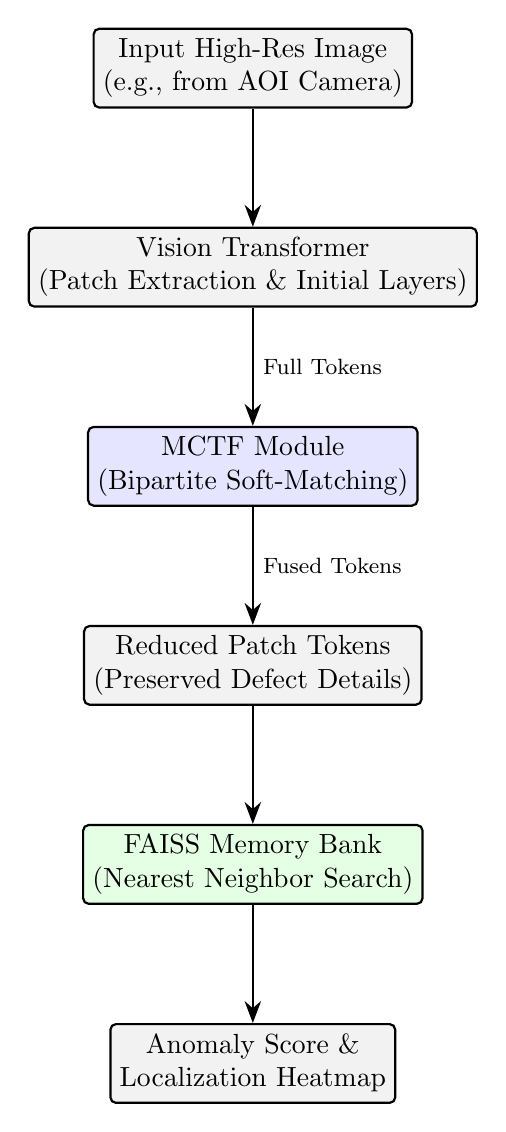
\begin{tikzpicture}[
        node distance=1.5cm and 1cm,
        box/.style={rectangle, draw=black, thick, minimum width=3.5cm, minimum height=1cm, align=center, fill=gray!10, rounded corners=2pt},
        arrow/.style={-{Stealth[scale=1.2]}, thick}
    ]
        % Nodes
        \node[box] (input) {Input High-Res Image \\ (e.g., from AOI Camera)};
        \node[box, below=of input] (vit) {Vision Transformer \\ (Patch Extraction \& Initial Layers)};
        \node[box, below=of vit, fill=blue!10] (mctf) {MCTF Module \\ (Bipartite Soft-Matching)};
        \node[box, below=of mctf] (fused) {Reduced Patch Tokens \\ (Preserved Defect Details)};
        \node[box, below=of fused, fill=green!10] (memory) {FAISS Memory Bank \\ (Nearest Neighbor Search)};
        \node[box, below=of memory] (output) {Anomaly Score \& \\ Localization Heatmap};

        % Arrows
        \draw[arrow] (input) -- (vit);
        \draw[arrow] (vit) -- node[right, font=\footnotesize] {Full Tokens} (mctf);
        \draw[arrow] (mctf) -- node[right, font=\footnotesize] {Fused Tokens} (fused);
        \draw[arrow] (fused) -- (memory);
        \draw[arrow] (memory) -- (output);
    \end{tikzpicture}
    \caption{High-Level Architecture of DefectLens integrating MCTF.}
    \label{fig:architecture}
\end{figure}

\section{References and Core Ideas}
This project heavily builds upon the novel token fusion concepts introduced in recent computer vision literature. Specifically, the core token reduction algorithm is inspired by the work of Lee et al. \cite{lee2023multi}. Their proposed "one-step-ahead attention" acts as an invaluable mechanism for informativeness, allowing the network to proactively protect tokens that will be highly attended to in subsequent layers, which is crucial for preserving the visibility of microscopic defects during industrial inspection.

\begin{thebibliography}{9}
\bibitem{lee2023multi}
Sanghyeok Lee, Joonmyung Choi, and Hyunwoo J. Kim,
\textit{``Multi-criteria Token Fusion with One-step-ahead Attention for Efficient Vision Transformers,''}
Department of Computer Science and Engineering, Korea University.
Emails: \{cat0626, pizard, hyunwoojkim\}@korea.ac.kr.
\end{thebibliography}

\end{document}
